\documentclass[UTF8]{ctexart}

\usepackage{subfigure}
\usepackage{listings}
\usepackage{color}
\usepackage{shapepar}
\usepackage{bbm}
\usepackage{graphicx}
\usepackage{amsmath}
\usepackage{CJKfntef}

\definecolor{dkgreen}{rgb}{0,0.6,0}
\definecolor{gray}{rgb}{0.5,0.5,0.5}
\definecolor{mauve}{rgb}{0.58,0,0.82}

\lstset{ %
  language=Octave,                % the language of the code
  basicstyle=\footnotesize,           % the size of the fonts that are used for the code
  numbers=left,                   % where to put the line-numbers
  numberstyle=\tiny\color{gray},  % the style that is used for the line-numbers
  stepnumber=2,                   % the step between two line-numbers. If it's 1, each line 
                                  % will be numbered
  numbersep=5pt,                  % how far the line-numbers are from the code
  backgroundcolor=\color{white},      % choose the background color. You must add \usepackage{color}
  showspaces=false,               % show spaces adding particular underscores
  showstringspaces=false,         % underline spaces within strings
  showtabs=false,                 % show tabs within strings adding particular underscores
  frame=single,                   % adds a frame around the code
  rulecolor=\color{black},        % if not set, the frame-color may be changed on line-breaks within not-black text (e.g. commens (green here))
  tabsize=2,                      % sets default tabsize to 2 spaces
  captionpos=b,                   % sets the caption-position to bottom
  breaklines=true,                % sets automatic line breaking
  breakatwhitespace=false,        % sets if automatic breaks should only happen at whitespace
  title=\lstname,                   % show the filename of files included with \lstinputlisting;
                                  % also try caption instead of title
  keywordstyle=\color{blue},          % keyword style
  commentstyle=\color{dkgreen},       % comment style
  stringstyle=\color{mauve},         % string literal style
  escapeinside={\%*}{*)},            % if you want to add LaTeX within your code
  morekeywords={*,...}               % if you want to add more keywords to the set
}










\usepackage{underscore}
\usepackage{fancyhdr}
\usepackage{extramarks}
\usepackage{amsmath}
\usepackage{amsthm}
\usepackage{amsfonts}
\usepackage{tikz}
\usepackage[plain]{algorithm}
\usepackage{algpseudocode} 
\usepackage{graphicx}
\usepackage{dsfont}
\usepackage{listings}
\lstset{language=Matlab}%代码语言使用的是matlab
\lstset{breaklines}%自动将长的代码行换行排版
\lstset{extendedchars=false}%解决代码跨页时,章节标题,页眉等汉字不显示的问题
\usetikzlibrary{automata,positioning}

\topmargin=-0.45in
\evensidemargin=0in
\oddsidemargin=0in
\textwidth=6.5in
\textheight=9.0in
\headsep=0.25in

\linespread{1.1}

\pagestyle{fancy}
\lhead{\hmwkAuthorName}
\rhead{\hmwkClass \:\hmwkTitle}
\cfoot{\thepage}

\renewcommand\headrulewidth{0.4pt}
\renewcommand\footrulewidth{0.4pt}

\setlength\parindent{0pt}


\newcommand{\enterProblemHeader}[1]{
    \nobreak\extramarks{}{问题\arabic{#1} continued on next page\ldots}\nobreak{}
    \nobreak\extramarks{问题 \arabic{#1} (continued)}{Problem \arabic{#1} continued on next page\ldots}\nobreak{}
}

\newcommand{\exitProblemHeader}[1]{
    \nobreak\extramarks{问题 \arabic{#1} (continued)}{Problem \arabic{#1} continued on next page\ldots}\nobreak{}
    \stepcounter{#1}
    \nobreak\extramarks{问题 \arabic{#1}}{}\nobreak{}
}

\setcounter{secnumdepth}{0}
\newcounter{partCounter}
\newcounter{homeworkProblemCounter}
\setcounter{homeworkProblemCounter}{1}
\nobreak\extramarks{ \arabic{homeworkProblemCounter}}{}\nobreak{}

\newenvironment{homeworkProblem}{
   %\section{ \arabic{homeworkProblemCounter}}
   %\setcounter{partCounter}{1}
    \enterProblemHeader{homeworkProblemCounter}
}{
    \exitProblemHeader{homeworkProblemCounter}
}


\newcommand{\hmwkTitle}{背包问题}
\newcommand{\hmwkClass}{MATLAB}
\newcommand{\hmwkClassTime}{}
\newcommand{\hmwkAuthorName}{郭龙昕,江诗毅,胡进}
\title{
    \vspace{2in}
    \textmd{\textbf{\hmwkClass:\ \hmwkTitle}}\\
    \vspace{0.1in}\large{\textit{ \hmwkClassTime}}
    \vspace{3in}
}
\author{\textbf{\hmwkAuthorName}}

\begin{document}

\maketitle

\pagebreak

\begin{homeworkProblem}

\section{任务一}
\subsection{实现思路}
实现思路:将求g(x)的最大值转换成求一个个小问题,背包容量从0到x逐步求出当前容量下的最优值(并且将子问题的最优选品方案存储起来),这样逐一迭代就能给出g(x)的最优值及其选品方案。

步骤:
\begin{itemize}
	\item 预分配内存:一个\( 1×(x+1) \)一维数组resultArr用来存储子问题的最优值,一个\( (x+1)×n \)二维数组s用来存储每个子问题的选品方案。
	\item 从0迭代到x,逐一选择比当前背包容量小的物品放入(或者不选任何物品)。将该物品的价值 加上当前容量减去该物品重量 这个子问题的最优值。
	\item 去掉重选,如果选择了一物品,并且该物品在子问题进行了选择,那么就不考虑该种方案。
	\item 从上述方案中选择价值最大的方案,这就是当前背包容量下的最优选品方案。
    \item 这样,最优值resultArr(x),最优的决策方案就是s(x,:)。
\end{itemize}
\subsection{具体实现}
下面分别给出伪代码和具体的代码

\textit{伪代码}
\begin{lstlisting}
预分配内存resultArr,s
for i=1 to x
    resultArr(i+1) = resultArr(i);  % 这就是不选物品的最优值。
    s(i+1,:) = s(i,:);  % 更改最优方案。
	
    % 找到所有重量比x小并且前面没有用到的物品的索引
    for j = 重量比i小的物品索引
        if 物品在前面用过
        continue;
    end

    % 比较选出价值最大的方案。
    if 当前的方案比之前的优
        % 更新方案
        resultArr(i+1) = v(j) + resultArr(i-w(j)+1);
        s(i+1,:) = s(i-w(j)+1,:); 
        s(i+1,j) = 1;
\end{lstlisting}

\textit{程序:knapsack.m}
\begin{lstlisting}
function [plan,opt] = knapsack(v,w,x)
%knapsack 浣跨敤鍔ㄦ�瑙勫垝姹傝В0-1鑳屽寘闂
%
%杈撳叆锛�%   v(vector) : 姣忎釜鐗╁搧鐨勪环鍊�%   w(vector) : 姣忎釜鐗╁搧鐨勯噸閲�%   x(vector) : 鑳屽寘鐨勫閲�%
%杈撳嚭锛�%   plan(vector) : 閫昏緫1鎴栬�閫昏緫0鍚戦噺锛岃〃绀烘槸鍚﹂�鎷╄鐗╁搧
%   opt(number) : 鏈�紭鐨勭墿鍝佷环鍊�
leng = length(v);
resultArr = zeros(1,x+1);  % g(x)鐨勭粨鏋�s = zeros(x+1,leng);  % 璺嚎

for i = 1:x
    % 璧嬩竴涓垵鍊�
    resultArr(i+1) = resultArr(i);
    s(i+1,:) = s(i,:);
    
    % 涓�釜瀛樻斁绗簩澶х殑 鏁扮粍
    %tem = zeros(1,length(v));
    for j = find(w<=i)  % 鎵惧埌鎵�湁閲嶉噺姣攛灏忕殑绱㈠紩  骞朵笖鍓嶉潰娌℃湁鐢�
        if ismember(j,find(s(i-w(j)+1,:) == 1) )
           continue;
        end 
        if v(j) + resultArr(i-w(j)+1) > resultArr(i+1)
            resultArr(i+1) = v(j) + resultArr(i-w(j)+1);
            s(i+1,:) = s(i-w(j)+1,:); 
            s(i+1,j) = 1;
        end
    end
end


plan = s(i+1,:);
opt = resultArr(x+1);

end
\end{lstlisting}
\subsection{正确性测试}
为了较好的验证算法的正确性,我使用了DP1与DP3(任务3中的动态规划)做对比,(见test.m),发现它们给出的解答在少数情况下是不相同的。

例如,当

重量向量为[24    41    22    32    33    43    21    18     5     3    16    28    24     4    41     1    28    41    22    34]

价值向量为[4    29    19    27    26     7    32    17    14     1    26    15    11    37    32    17    20     6    27    27]

DP1得到的解为305,DP3得到的最优解为306,也就是说其中一个DP存在问题。下一节阐述DP1的问题所在。

我们发现是任务一的代码存在问题:

\subsection{改进方法}
前面说到,DP1得到的最优解有问题,于是重新check代码,发现这个DP方程对0-1背包问题来说有一个问题,那就是在后面选择物品的时候,可能该物品已经在子问题中选择过了,而我采取的办法是直接将这种方案从整个可行解集中去掉。这样就带来错误。正确的做法是将这种重复选择的物品的重量从容量中减去,并且在子问题中也不考虑这种物品。这样就不符合DP方程的定义了。

于是更改0-1背包问题为0-n背包问题,也就是说每个物品可以选择多个,而不是一个,同样最优方案用一维数组表示,第i个位置的值表示选择了该物品几次。

\textit{更改后的代码}
\begin{lstlisting}
function [plan,opt] = correctKnapsack(v,w,x)
%correctKnapsack    纠正1中的0-1背包问题解法,改为物品个数无限。
%
%输入:
%   v(vector) : 每个物品的价值
%   w(vector) : 每个物品的重量
%   x(vector) : 背包的容量
%
%输出:
%   plan(vector) : 表示第i个物品选了几个
%   opt(number) : 最优的物品价值
    leng = length(v);
    resultArr = zeros(1,x+1);  % g(x)的结果
    s = zeros(x+1,leng);  % 路线
    
    for i = 1:x
        % 赋一个初值 
        resultArr(i+1) = resultArr(i);
        s(i+1,:) = s(i,:);
        for j = find(w<=i)  % 找到所有重量比x小的索引
            if v(j) + resultArr(i-w(j)+1) > resultArr(i+1)
                resultArr(i+1) = v(j) + resultArr(i-w(j)+1);
                s(i+1,:) = s(i-w(j)+1,:); 
                s(i+1,j) = s(i+1,j) + 1;
            end
        end
    end    
    plan = s(i+1,:);
    opt = resultArr(x+1);
end
\end{lstlisting}
\subsection{改进后的代码正确性测试}
同样针对上面的例子:

重量向量为[24    41    22    32    33    43    21    18     5     3    16    28    24     4    41     1    28    41    22    34]

价值向量为[4    29    19    27    26     7    32    17    14     1    26    15    11    37    32    17    20     6    27    27]

对于容量25,得出的结果为:[0     0     0     0     0     0     0     0     0     0     0     0     0     0     0    25     0     0     0     0],很容易验证这是正确的。

\subsection{算法效率分析}
算法的时间复杂度为 \(O(nx)\),其中n为物品的个数,x为背包的容量大小。

绘制时间随规模--nx衡量的散点图,并用一次函数拟合,结果如下图(图1,图2).

由图可知,该算法的时间复杂度能较好的使用\( O(nx) \)来描述。
用伪代码的迭代语句中能够看出,首先是对1到x的背包容量进行了迭代,然后在每一种背包容量下对每一个物品进行了查找。共有n个物品,故算法的时间复杂度为\(O(n)\)。

内存开销,用到了一个\( 1×(x+1) \)一维数组,一个\( (x+1)×n \)二维数组,故空间复杂度为\( (x+1)(n+1)  \)

\begin{figure}[H] %[htbp]
	\centering


		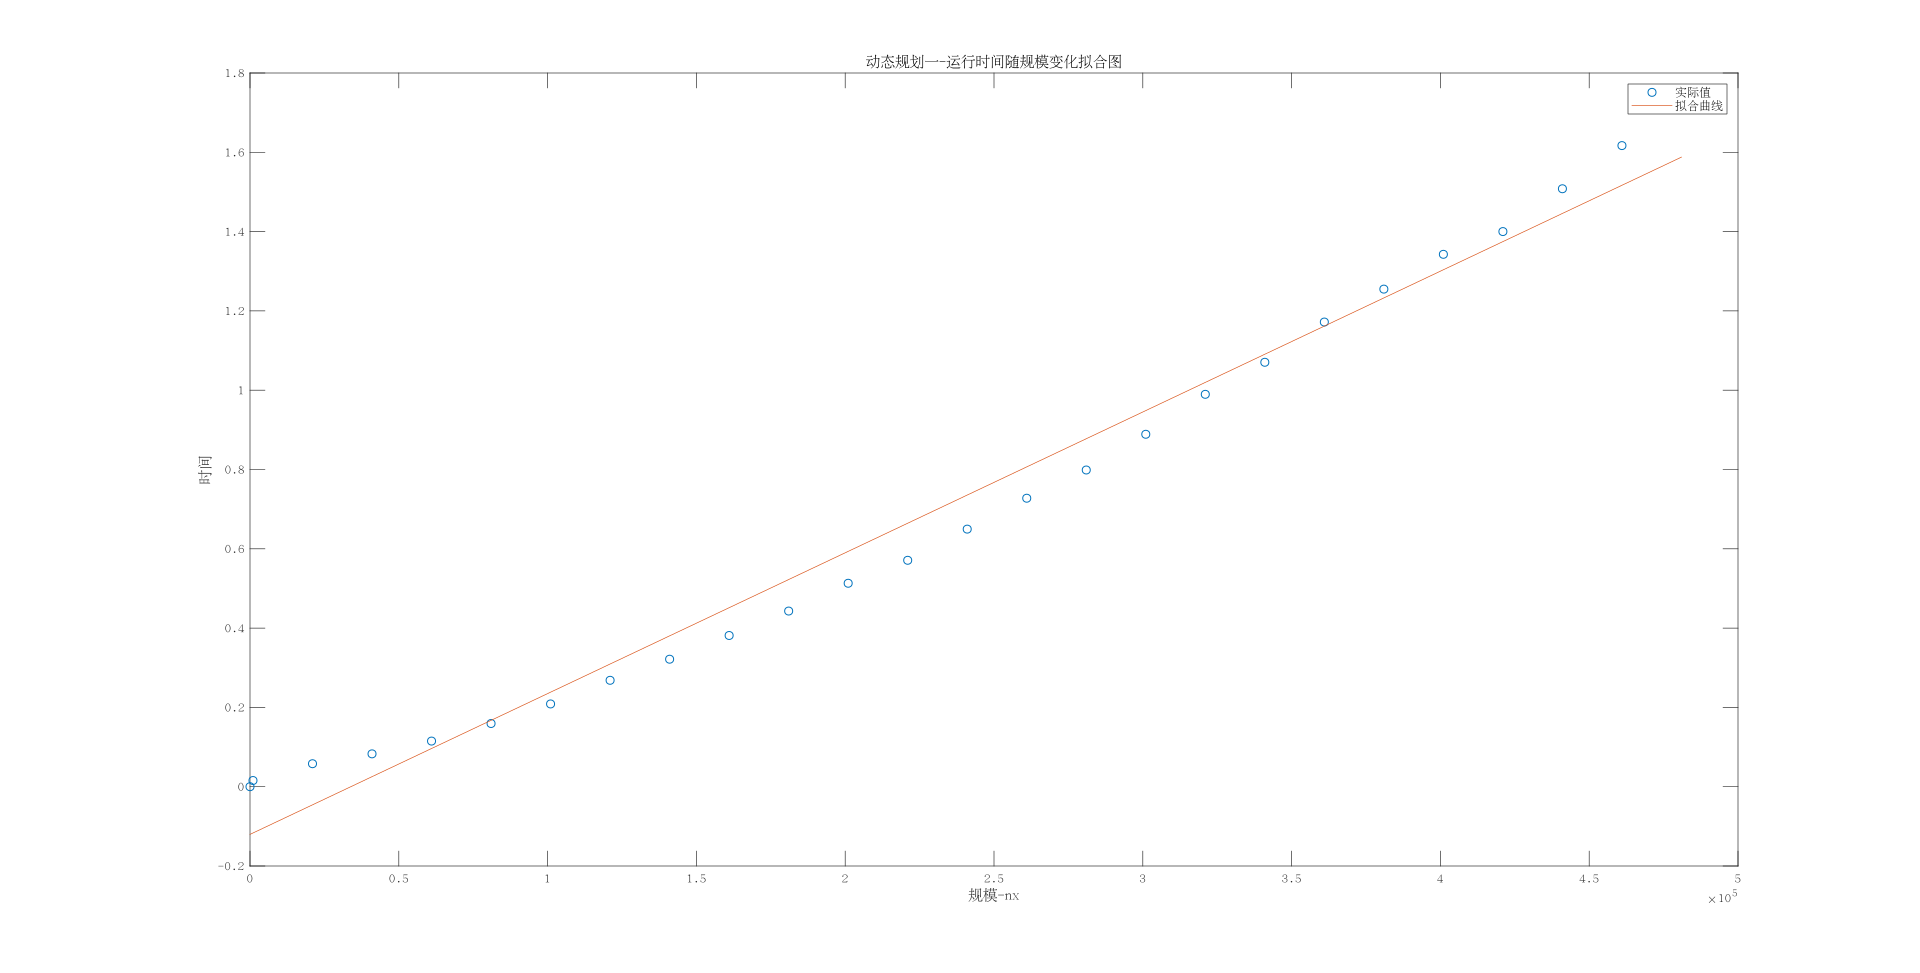
\includegraphics[width=10cm]{1.png}
		\caption{稀疏点拟合}
\end{figure}

\begin{figure}
		\centering
		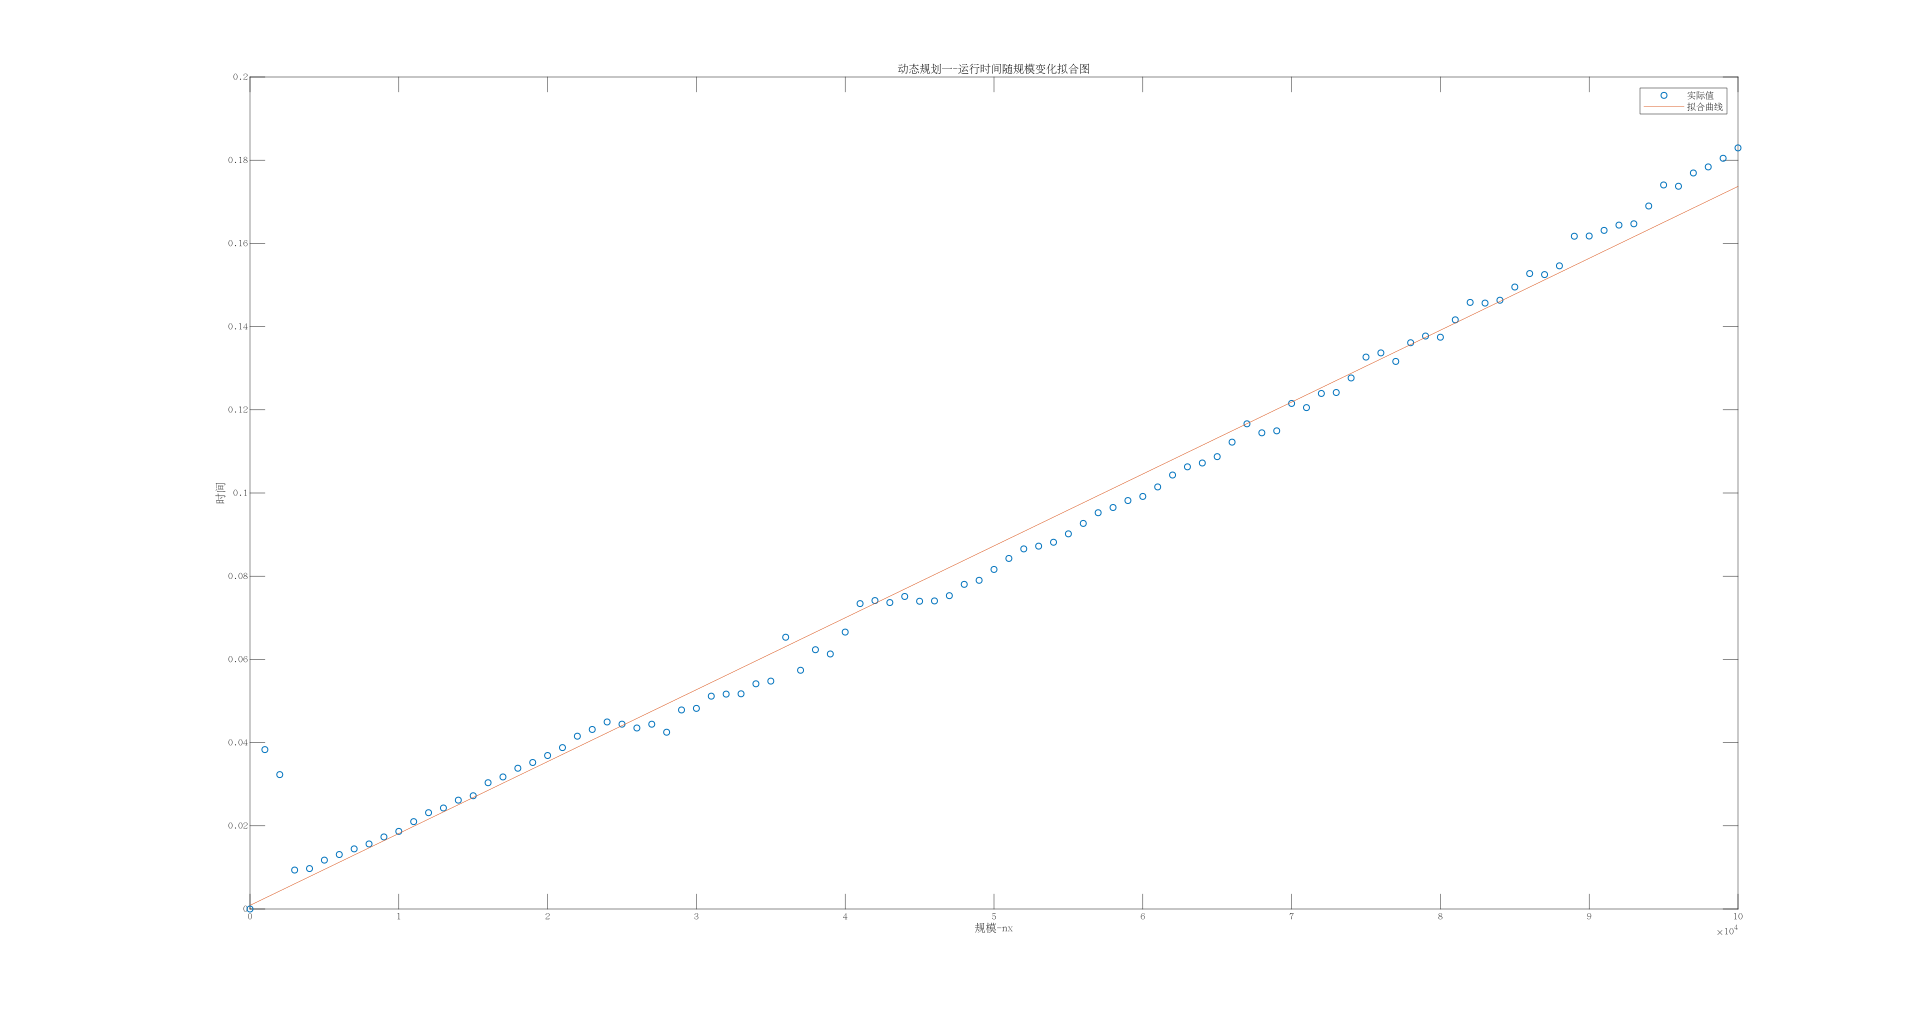
\includegraphics[width=10cm]{2.png}
		\caption{密集点拟合}
\end{figure}
\section{任务二}

\subsection{贪婪算法}
针对背包问题,一种很自然的想法就是先选择性价比最高的物品,也就是v/w最高的。但是这只是在当前看来是最优的选着,但是对于长远来说,可能存在浪费背包容量的问题,所以这只是一种近似的解法。

\subsection{实现思路}
步骤:
\begin{itemize}
    \item 将物品按找v/w从大到小排序。
    \item 选择当前背包剩余容量能装下的最大性价比的物品。
    \item 重复第二步,直到背包再也装不下任何物品。
\end{itemize}

\subsection{具体程序}
\begin{lstlisting}
function [plan,opt] = greedy(v,w,x)
%greedy 浣跨敤璐┆绠楁硶姹傝В0-1鑳屽寘闂鐨勮繎浼艰В銆�%
%杈撳叆锛�%   v(vector) : 姣忎釜鐗╁搧鐨勪环鍊�%   w(vector) : 姣忎釜鐗╁搧鐨勯噸閲�%   x(vector) : 鑳屽寘鐨勫閲�%
%杈撳嚭锛�%   plan(vector) : 閫昏緫1鎴栬�閫昏緫0鍚戦噺锛岃〃绀烘槸鍚﹂�鎷╄鐗╁搧
%   opt(number) : 鏈�紭鐨勭墿鍝佷环鍊�unit = v./w;
plan = zeros(1,length(w));
opt = 0;

i = find(unit==max(unit));
i = i(1);

while x >= w(i)
    plan(i) = 1;
    opt = opt + v(i);
    x = x - w(i);
    unit(i) = 0;
    i = find(unit==max(unit));
    i = i(1);
end

end
\end{lstlisting}

\subsection{算法效率分析}
按照问题描述,由于所有的物品都只扫描了一次,所以算法的时间复杂度为\(O(n)\)。

启发的式的贪婪算法虽然得不到问题的最优解,但是其在问题规模较大的时候,能得到比较理想的结果,并且其时间复杂度相比与动态规划大幅降低了。

如下图:
\begin{figure}[H] %[htbp]
    \centering
        \includegraphics[width=10cm]{10.png}
        \caption{对比}
\end{figure}

\section{任务三}

\subsection{实现思路}
步骤:
\begin{itemize}
    \item 预分配内存:使用一个n×(x+1)二维数组temp来存储所有子问题的最优值,以及一个n×(x+1)的0-1二维数组s来存储当前最优方案下是否选择了新增的物品。
    \item 从只有一个物品开始迭代,同时背包容量也从0开始迭代直到x为止。
    \item 在当前物品集合下,当前背包容量下做出是否选择当前物品的决策。并且记录下来
    \item 最后的temp(n,x+1)就是最优值,决策方案根据s给出,具体步骤如下。
\end{itemize}

根据s给出决策方案步骤:
\begin{itemize}
    \item 从s(n,x+1)开始,如果为1,证明选择了第n个物品。如果为0,证明没选。
    \item 如果上一步为1,那么跳到 s(n-1,x+1-v(n)) ,看它为1还是0。如果上一步为0,跳到s(n-1,x+1)进行判断。
    \item 重复上述步骤,直到全部判断完毕,这样就得出了最优方案。
\end{itemize}

\subsection{具体程序}
\textit{程序:knapsack.m}
\begin{lstlisting}
function [plan,opt] = knapsack(v,w,x)
%knapsack 浣跨敤鍔ㄦ�瑙勫垝姹傝В0-1鑳屽寘闂
%
%杈撳叆锛�%   v(vector) : 姣忎釜鐗╁搧鐨勪环鍊�%   w(vector) : 姣忎釜鐗╁搧鐨勯噸閲�%   x(vector) : 鑳屽寘鐨勫閲�%
%杈撳嚭锛�%   plan(vector) : 閫昏緫1鎴栬�閫昏緫0鍚戦噺锛岃〃绀烘槸鍚﹂�鎷╄鐗╁搧
%   opt(number) : 鏈�紭鐨勭墿鍝佷环鍊�
leng = length(v);
resultArr = zeros(1,x+1);  % g(x)鐨勭粨鏋�s = zeros(x+1,leng);  % 璺嚎

for i = 1:x
    % 璧嬩竴涓垵鍊�
    resultArr(i+1) = resultArr(i);
    s(i+1,:) = s(i,:);
    
    % 涓�釜瀛樻斁绗簩澶х殑 鏁扮粍
    %tem = zeros(1,length(v));
    for j = find(w<=i)  % 鎵惧埌鎵�湁閲嶉噺姣攛灏忕殑绱㈠紩  骞朵笖鍓嶉潰娌℃湁鐢�
        if ismember(j,find(s(i-w(j)+1,:) == 1) )
           continue;
        end 
        if v(j) + resultArr(i-w(j)+1) > resultArr(i+1)
            resultArr(i+1) = v(j) + resultArr(i-w(j)+1);
            s(i+1,:) = s(i-w(j)+1,:); 
            s(i+1,j) = 1;
        end
    end
end


plan = s(i+1,:);
opt = resultArr(x+1);

end
\end{lstlisting}

\subsection{正确性测试}
在任务一中已经证明,这里不再赘述

\subsection{算法效率分析}
从实现思路上来说,第一种只对背包的容量进行了“动态规划”,而第二种在对背包容量进行动态规划的同时,也对物品的种类进行了划分。所以针对第一种,我使用了一个一维数组存储最优值,对于第二种,使用了二维的数组。在求解决策方案上,对于第一种,直接将每个子问题的选品方案存在一个二维数组里面,对于第二种,我是从物品的角度来看,如果选择了当前迭代的物品,那么存1,否则存0.

空间复杂度:第一种使用一个一维数组,一个二维数组。第二种动态规划使用两个二维数组。故易知,第二种方案在空间上开销优于第一种。

时间复杂度:两种方案都近似于\(O(nx)\)。但在循环内部,第一种每一次都要查找所有物品,而第二种只用决策是否选择当前物品。故总的来说,第二种动态规划在时间上消耗比第一种少很多。由前面给出了图也看出,第一种的数量级为1,第二种的数量级为\(10^{-4}\)

下面给出图示验证。
\begin{figure}[H] %[htbp]
    \centering
        \includegraphics[width=10cm]{5.png}
        \caption{对比}
\end{figure}

\end{homeworkProblem}
\end{document}
